
\section{Stability}


\subsection{Critical Point (Node)}

\begin{tcolorbox}[colback=green!10,colframe=green!50!black,title=\textbf{Critical Point (Node)}]
Consider the following LTI:
\[
\dot{x} = f(\mathbf{x}, t)
\]
\(x_0\) is called a \textbf{Node}, or \textbf{Critical Point}, if \(f(x_0) = 0\).
\end{tcolorbox}

\subsection{Stability}
\begin{tcolorbox}
A system is \textbf{stable} if:
\[
\|x(0) - x_0 \| < \delta \quad \| x(t) -x_0\| < \epsilon
\]
\end{tcolorbox}

We can think of it as: if the starting point is in the $\delta$-neighborhood of the node $x_0$, 
the rest of the trajectory $x(t)$ is in the $\epsilon$-neighborhood of the node.

Or, the solutions starting from the $\delta$-sized ball do not diverge. 

\subsection*{Asymptotic Stability}

\begin{tcolorbox}
A system is \textbf{asymptotically stable} if:
\[
\|x(0) - x_0 \| < \delta \to \lim_{t \to \infty} x(t) = x_0 
\]
\end{tcolorbox}

For any initial point that lies in the \(\delta\)-sized ball, the trajectory will asymptotically approach the node (point $x_0$).
Or, the solutions starting from the \(\delta\)-sized ball, converge to the node. \\

\textbf{Lyapunov Stability:} A more general concept applicable to all systems, ensuring that trajectories remain close to the equilibrium point if they start close enough.
Assymptotically stable systems are stable in the sense of Lyapunov.

An equilibrium point which is Lyapunov stable but not asymptotically stable is called marginally stable point


\textbf{Marginal Stability:} Specific to LTI systems and defined by the eigenvalues' locations. It implies that the system's response neither grows unbounded nor decays, often resulting in sustained oscillations.


\begin{center}
    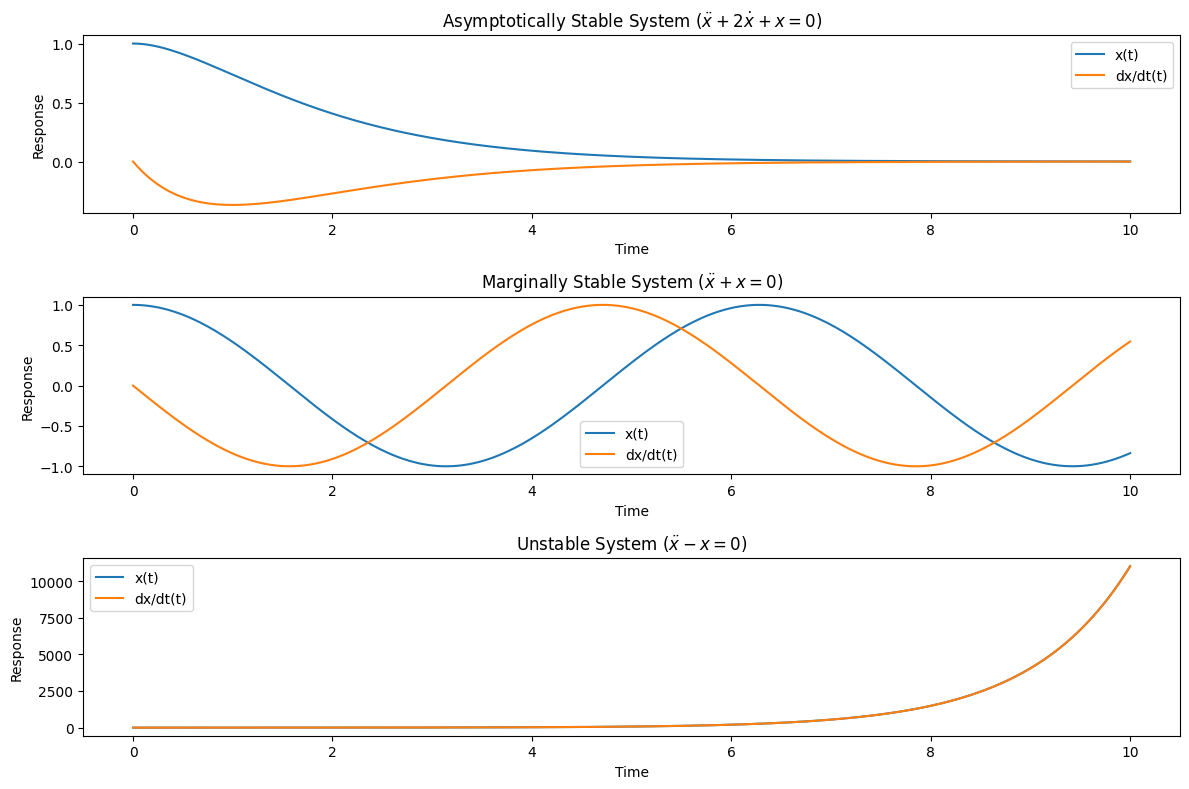
\includegraphics[scale=0.42]{images/stability_plots.png}
\end{center}

\subsection{Stability of autonomous LTI}

\subsection*{\underline{Autonomous Systems}}

A system is considered \underline{\textbf{autonomous}} if its evolution depends only on time.\\

\underline{Example}

\[
\mathbf{\dot{x}}=\mathbf{A}\mathbf{x} + \mathbf{B}\mathbf{u}
\]

\subsubsection{Diagonal matrices}

Let's introduce a trick for autonomous Linear Time-Invariant (LTI) systems.

First of all, recall the properties of a diagonal matrix and eigen-decomposition.
\begin{itemize}
    \item \textbf{Diagonal matrix}
        \[\mathbf{\dot{z}} = \mathbf{D}  \mathbf{z}\]
        \[
        \begin{cases}
            \dot{x}_1 = d_1 x_1 \\
            \dots \\
            \dot{x}_n = d_n x_n
        \end{cases}
        \]
        The solution of each of the equations is: \(x_i = C_i e^{d_i t}\).
        So, the system is asymptotically stable when for all \(i\), \(d_i < 0\). 
        The system is stable when \(d_i \leq 0\).
    \item \textbf{Eigen-decomposition}\\
        We can represent the matrix as \(A = VDV^{-1}\), where \(D\) is a diagonal matrix.
\end{itemize}

Given an autonomous Linear Time-Invariant (LTI) system, let's switch to the system with a diagonal matrix:
\[
\mathbf{\dot{x}} = \mathbf{A} \mathbf{x}
\]

\[
\mathbf{\dot{x}} = \mathbf{V} \mathbf{D} \mathbf{V}^{-1} \mathbf{x}
\]

\[
\mathbf{V}^{-1} \mathbf{\dot{x}} = \mathbf{V}^{-1} \mathbf{V} \mathbf{D} \mathbf{V}^{-1} \mathbf{x} = \mathbf{D} \mathbf{V}^{-1} \mathbf{x}
\]

Change of variables: \(\mathbf{z} = \mathbf{V}^{-1} \mathbf{x}\), \(\mathbf{\dot{z}} = \mathbf{D} \mathbf{z}\),

\[
\mathbf{V}^{-1} \mathbf{\dot{x}} = \mathbf{D} \mathbf{z}
\]


The system is asymptotically stable when for all the elements of \(D\) are \( < 0\). 
The system is stable when the elements of \(D\) are \(\leq 0\).  

\subsubsection{Upper triangular matrices}

\begin{tcolorbox}[colback=white]
    Eigenvalues of upper triangular matrices are the diagonal elements.
\end{tcolorbox}
    

\subsubsection{General case}

Consider the LTI:
\[\mathbf{\dot x} = \mathbf{A} \mathbf{x}\]

\begin{tcolorbox}[colback=green!10,colframe=green!50!black]
    The system is called \textbf{stable} iff real parts of eigenvalues of A are non-positive.
\end{tcolorbox}

\begin{tcolorbox}[colback=green!10,colframe=green!50!black]
    The system is called \textbf{asymptotically stable} iff real parts of eigenvalues of A are  strictly negative. 
\end{tcolorbox}

\subsection{Pole placement method}

\textbf{Pole placement} is a fundamental and useful method for achieving stabilization in control systems. With this method, we can manually choose the locations of the system's poles, which correspond to the points where the system would ideally converge to.

\begin{center}
    \underline{\textbf{Example:}}

\end{center}
Check stability of the system and in case the system is unstable, stabilize it using the Pole Placement method:

\[
\begin{bmatrix}
\dot{x} \\
\ddot{x}
\end{bmatrix} = 
\begin{bmatrix}
0 & 1  \\
2 & -1  
\end{bmatrix}
\begin{bmatrix}
x \\
\dot{x} 
\end{bmatrix} + 
\begin{bmatrix}
1 \\
0 
\end{bmatrix} u
\]

Let's check the eigenvalues:
\[
\text{det} (A - \lambda I) = 0
\]
\[
\text{det}\left(\begin{bmatrix}-\lambda & 1 \\ 2 & -1 - \lambda\end{bmatrix}\right) = \lambda(1 + \lambda) -2 = \lambda^2 + \lambda - 2
\]
Eigenvalues \( \lambda_1, \lambda_2 = -2, 1 \).
Since one of the roots is positive, the system is unstable. Let \( U = -K \),
Then, \( \dot{x} = Ax - BKx \).

Consider the matrix \( A-BK \):
\[
A-BK = \begin{bmatrix}0 & 1 \\ 2 & -1\end{bmatrix} - \begin{bmatrix}1 \\ 0\end{bmatrix}\begin{bmatrix}k_1 & k_2\end{bmatrix} = \begin{bmatrix}0 & 1 \\ 2 & -1\end{bmatrix} - \begin{bmatrix}k_1 & k_2 \\ 0 & 0\end{bmatrix} = \begin{bmatrix}-k_1 - \lambda & 1-k_2 \\ 2 & -1-\lambda\end{bmatrix}
\]

Let's choose negative eigenvalues \( -1 \) and \( -2 \).
Solving the system of two equations, we get \( k_1 = 2 \), \( k_2 = 1 \).
And the control law will be:
\[
u = - Kx = \begin{bmatrix}2 & 1\end{bmatrix}x
\]
